
On obtient la pente d'une route en calculant le quotient du dénivelé (c'est-à-dire du déplacement vertical) par
le déplacement horizontal correspondant. Une pente s'exprime sous forme d'un pourcentage.

\medskip

\parbox{0.45\linewidth}{Sur l'exemple ci-contre, la pente de la route est :

\medskip

$\dfrac{\text{dénivelé}}{\text{déplacement horizontal}} =  \dfrac{15}{120} = 0,125 = 12,5\,\%$.}
\hfill \parbox{0.52\linewidth}{ 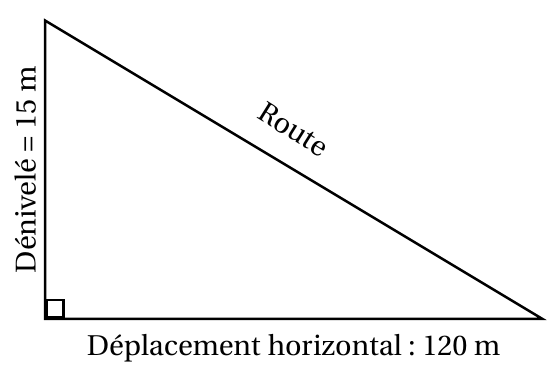
\includegraphics[scale=0.4]{TR-217-0.png}
}

\bigskip

Classer les pentes suivantes dans l'ordre décroissant, c'est-à-dire de la pente la plus forte à la pente la moins forte.

\begin{center}
\begin{tabularx}{\linewidth}{|m{6cm}|X|}\hline
Route descendant du château des  Adhémar, à Montélimar.
\vspace{1,75cm}&  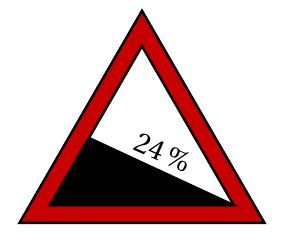
\includegraphics[scale=0.5]{TR-217-1.png} \\ \hline
Tronçon d'une route descendant du col 
 du Grand Colombier (Ain).\vspace{1,75cm}&\psset{unit=0.6cm}
 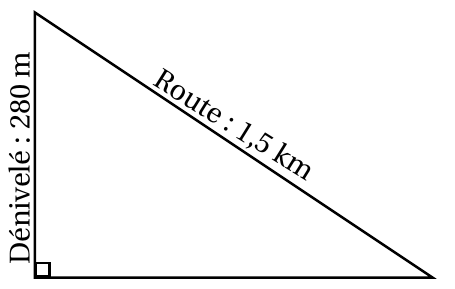
\includegraphics[scale=0.5]{TR-217-2.png} \\ \hline
Tronçon d'une route descendant de l'Alto
de l'Angliru (région des Asturies,
Espagne).\vspace{1,75cm}& 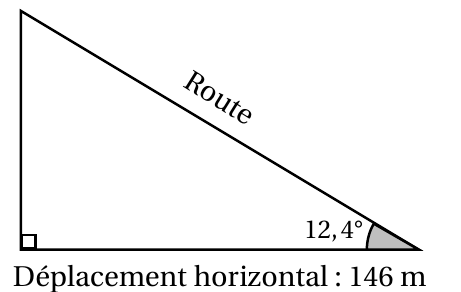
\includegraphics[scale=0.5]{TR-217-3.png} \\ \hline
\end{tabularx}
\end{center}




